\section{A description of \acs{EsPy}}

\subsection{Why \textsc{Python}?}
There a number of reasons why \textsc{Python} was the chosen programming
language for \ac{EsPy}:
\begin{itemize}
    \item It has a large user-base, particularly within the scientific
        community.
    \item The \textsc{SciPy} ecosystem~\cite{Virtanen2020}, including the packages
        \textsc{NumPy}~\cite{Harris2020} and
        \textsc{Matplotlib}~\cite{Hunter2007} enables
        high-performance scientific computation and data visualisation in
        \textsc{Python}, despite the language's reputation for slow speed.
    \item Being a scripting language with user-friendly syntax makes
        \textsc{Python} ideal for exploring datasets in a step-by-step fashion.
        This is useful in the context of \ac{EsPy}, as a user will want to
        (a) inspect and pre-process the data of interest,
        (b) determine the regions they wish to estimate and set up the
        estimation routine,
        and (c) output and inspect the result.
        This can be achieved easily by ``hacking'' and re-running
        \textsc{Python} scripts or by using notebook environments, such as
        \textsc{Jupyter}.
    \item It is free and open-source, as opposed to well-known scientific
        computing platforms such as \textsc{Matlab} and \textsc{Mathematica}.
    \item \textsc{Python} supports sophisticated object-oriented programming
        features, including multiple levels of inheritance. This is exploited in
        \ac{EsPy} to facilitate the creation of numerous objects designed with
        specific \ac{NMR} data types in mind (\textit{vide infra}).
\end{itemize}

Probably the largest disadvantage in using \textsc{Python} is its slow performance;
some of the features which makes \Python\ user-friendly lead to significant
runtime overheads\footnote{
    \Python is interpreted rather than compiled, dynamically typed rather
    than statically typed, and it relies on garbage collection for memory
    management, rather than requiring the programmer to do this manually. All
    of these features are slower than the alternatives which are mentioned;
    these alternatives feature in low-level languages like C, C++, and
    \textsc{Rust}.
}. While \textsc{NumPy} provides
interfaces to run fast computations with pre-compiled C-code, a significant
performance benefit would likely be realised if a low-level compiled language
like C, C++, or \textsc{Rust} were used instead (this is discussed more in
\cref{sec:future-work}). While this may be so, the
development time in writing programs with these higher-performance languages is
typically a lot greater those with a higher level of abstraction
like \textsc{Python}.

\subsection{Estimator Objects}
\label{subsec:estimator-objects}
\begin{figure}
    \centering
    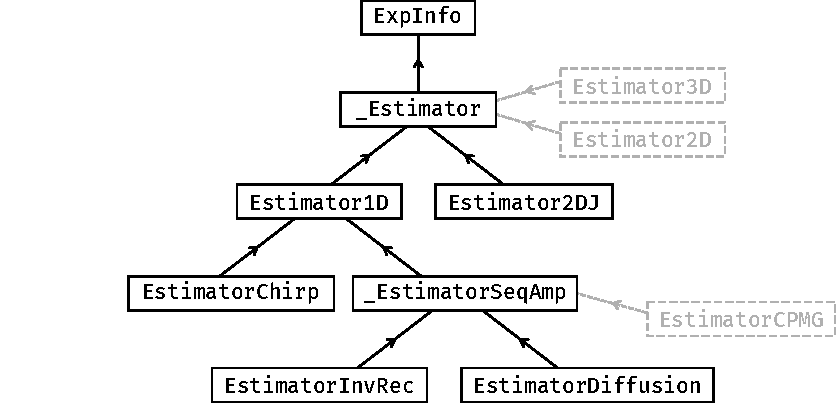
\includegraphics{inheritance_tree/inheritance_tree.pdf}
    \caption[
        An inheritance tree of the estimation classes in the \acs{EsPy} package.
    ]{
        An Inheritance tree of the estimation classes in the \acs{EsPy} package.
        Arrows are directed from child classes to the parent class they
        directly inherit from. Classes in grey are objects that could be added
        to the \ac{API} in the future.
    }
    \label{fig:inheritance}
\end{figure}
The fundamental user-facing objects (\emph{classes}) that \ac{EsPy} provides are
called \emph{estimators}.
Instances of these estimator classes contain relevant pieces of data called
\emph{attributes} (e.g. the \ac{FID} and experiment parameters including the
spectral width and transmitter offset), as well as \emph{methods} which perform
routines applicable to the class like estimation and result figure generation.
Thanks to \textsc{Python}'s support for multiple levels of inheritance, it is
possible to build numerous objects with certain shared attributes and methods,
but which also possess bespoke features that are solely of relevance to
the type of \ac{NMR} data being considered. As an example, only the
\texttt{Estimator2DJ} object possesses a method called \texttt{cupid\_spectrum},
which returns the \ac{FT} of the \ang{-45} signal.
\Cref{fig:inheritance} provides an inheritance
diagram, outlining the relationship between different estimators in
\ac{EsPy}. Basic overviews of each of these are as follows:
\begin{itemize}
    \item \textbf{\textbf{\texttt{ExpInfo}}} stores the parameters that were
        used to run a particular \ac{NMR} experiment. \texttt{ExpInfo} also has
        methods for the generation of the timepoints and chemical shifts sampled
        based on these parameters, and for producing synthetic \acp{FID} if a
        set of signal parameters is provided.
    \item \textbf{\texttt{\_Estimator}} inherits experimental parameters from
        \texttt{ExpInfo}, but also possesses the \ac{NMR} dataset itself.
        This class is designed to contain the functionality which can be
        generalised across all \ac{NMR} data types supported by \ac{EsPy}. It
        does not possess all the features necessary to be useful as a standalone
        object, and as such the user is not supposed to use it directly (such
        an object is often referred to as an abstract class; this is emphasised
        by starting the object's name with an underscore).
    \item \textbf{\texttt{Estimator1D}} handles conventional \ac{1D} datasets,
        such as those in \cref{sec:evaluation}.
    \item \textbf{\texttt{\_EstimatorSeqAmp}} is an abstract class
        which enables the estimation of sequential \ac{1D} datasets such as those
        described in \cref{sec:seq}. Analysis of a given dataset varies depending on
        the type of experiment considered, since the function used for
        fitting amplitudes (\cref{tab:seq-equations}) and the means by
        which that data should be imported varies. As such, this is not
        designed for direct use; one of the classes which inherit it should be
        used instead. Under the hood, \texttt{\_EstimatorSeqAmp} stores a
        number of \texttt{Estimator1D} objects; each of these contains one
        of the \acp{FID} in the sequential dataset. Estimation simply comprises
        iterating through these estimators, giving the parameter estimate of
        the previous estimator to next as its initial guess for \ac{NLP}.
    \item \textbf{\texttt{EstimatorInvRec}} is for the estimation of inversion
        recovery datasets.
    \item \textbf{\texttt{EstimatorDiffusion}} is for the estimation of
        diffusion datasets.
    \item \textbf{\texttt{EstimatorChirp}} is for the estimation of \acp{FID}
        acquired using single-chirp excitation, as described in \cref{sec:bbqchili}.
    \item \textbf{\texttt{Estimator2DJ}} is for the estimation of \ac{2DJ} data.
        This class provides features to generate pure shift spectra and
        assign multiplet structures using \ac{CUPID}, as described in
        \cref{chap:cupid}.
\end{itemize}

Other estimator objects which are yet to be implemented, but are potential
future additions to the package are also depicted in the inheritance diagram.
\texttt{EstimatorCPMG} would enable the analysis of \ac{CPMG}/\ac{PROJECT} datasets,
while \texttt{Estimator2D} and \texttt{Estimator3D} would be
for the estimation of datasets comprising sets of \ac{2D} or \ac{3D} amplitude-
or phase-modulated \acp{FID}, respectively. A discussion of the feasibility of
implementing the \ac{2D} and \ac{3D} estimators is given in
\cref{sec:future-work}.

\subsection{Example Usage}
\mylisting{python3}{code_listings/cupid_example.py}{%
    The \textsc{Python} script used to produce the camphor \acs{CUPID} result
    (\cref{fig:camphor-cupid}).
}{
    The \textsc{Python} script used to produce the camphor \acs{CUPID} result
    (\cref{fig:camphor-cupid}).
}{lst:espy-example}
\cref{lst:espy-example} provides an example of \ac{EsPy} being used for the
consideration of \ac{2DJ} data; it is similar to the script which was to
generate the camphor result presented in \cref{fig:camphor-cupid}.  The script
carries out the following:
\begin{enumerate}
    \item An \texttt{Estimator2DJ} object is initialised, which imports and stores
        the \textsc{Bruker}-formatted camphor dataset, located at the path
        \path{$HOME/data/camphor/1}\footnote{
            \path{$HOME} denotes the current user's home directory on a
            UNIX-based system. In many scenarios, the tilde symbol
            (\mintinline{text}{~})
            can be used to denote the home directory as well.
        }
        (Line \ref{ln:newbruker}).
    \item The \ac{2DJ} \ac{FID} is pre-processed to ensure it is phased and
        features a flat spectral baseline (Lines \ref{ln:phase} and
        \ref{ln:baseline}).
    \item The regions of interest are defined, in units of
        \unit{\partspermillion} (Lines \ref{ln:regionstart} to
        \ref{ln:regionend}). Each region is given by a two-element tuple
        containing its left- and right-boundaries.
    \item For each region, parameter estimates are determined using the
        \mintinline{python}{Estimator2D.estimate} method, which constructs a filtered
        sub-\ac{FID}, and subsequently analyses it (Lines
        \ref{ln:estimatestart} to \ref{ln:estimateend}). Most arguments given
        are self-explanatory; \mintinline{python}{nlp_trim} can be set to
        truncate the sub-\ac{FID} in the direct dimension, to reduce the
        computational burden on the \ac{NLP} routine. By default
        the \ac{MDL} is used for model order selection.
    \item After estimation is complete, the estimator object is saved to a byte
        stream using \textsc{Python}'s ``pickling'' protocol~\cite{pickle} (Line
        \ref{ln:pickle}).
        This enables the estimator to be recovered at a later time.
    \item A pure shift spectrum is produced via the \ang{-45} signal, and
        stored to the path \path{$HOME/data/camphor/2} in a format that enables
        it to be read by software that supports \textsc{Bruker} datasets,
        such as \textsc{TopSpin} (Line \ref{ln:writecupid}).
    \item Finally, a figure depicting the estimation result is produced (making
        use \textsc{Matplotlib}) and saved (Lines \ref{ln:makefig} and
        \ref{ln:savefig}). The form the figure takes is reminiscent of
        \cref{fig:camphor-cupid}, though a lot of aesthetic customisation has
        been applied to the latter.
\end{enumerate}
